\section{Synthetic evaluation with overdetermination and undercutting}
\label{sub:synthetic}


In this evaluation, we build off the existing counterexamples to the but-for clause as an explanation tool. Recall that the  initial intuition one might have is the following:

\begin{quote}
$X=x$ is responsible for $Y=y$ just in case $Y$ would have been different had we intervened on $X$ to be different, i.e. if $Y_{x'} = y'$ for some $x' \neq x, y' \neq y$.
\end{quote}

A typical counterexample to this is cast in terms of categorical variables \cite{actualCausalityHalpern}:

\begin{quote} Sally and Billy pick up stones and throw them at a bottle. Sally’s stone gets there first, shattering the bottle. Both throws are perfectly accurate, so Billy’s stone would have shattered the bottle had it not been preempted by Sally’s throw. The intuition is that Sally's throw is responsible for the shattering, but not so Billy's. However, it is false that had Sally not thrown the stone, the bottle would not have shattered, so the simple counterfactual condition fails.
\end{quote}

What we want to investigate is the performance of responsibility attribution, using the same implementation as the one used in Appendix \ref{sub:amv}, following the discussion in Section \ref{sec:scaling}, in the context of a synthetic generalization of this problem. Suppose we use continuous variables in a model with a similar overdetermination and undercutting structure. Is the tool capable of meeting our expectations when it comes to responsibility attribution?

The answer is positive. We first introduce the model, introduce intuitive qualitative desiderata, and investigate their satisfaction for 500 local explanations, for events generated using the same generative process, with responsibility scores for all features estimated using one sample of size 5000.

The way we generalize is as follows. The input and output variables are continuous. The $A$ variables are like Sally's throw: they have an unblocked impact on the outcome. The $C$ variables are like Billy's throw: if their linear combination is high enough, they are active and can have an impact on the outcome. Otherwise, their impact is blocked. $B$ and $D$ are like `Sally hits' and `Bill hits', except continuous, and $E$ is some final outcome, except now we don't use a disjunction, but rather addition.


\begin{align*}
\text{For } i = 0, 1, 2: &  \\
&\quad A_i \sim \mathcal{N}(0, 1), \\
&\quad C_i \sim \mathcal{N}(0, 1), \\
\text{and}  & \\
 B & = 0 \cdot A_0 + 5 \cdot A_1 + 10 \cdot A_2, \\
 cs\_dot & = 0 \cdot C_0 + 5 \cdot C_1 + 10 \cdot C_2, \\
 cs\_win &= \mathbf{1}\{ cs\_dot > B \}, \\
 D & = cs\_dot \cdot cs\_win, \\
 E& = B + D.
\end{align*}


\noindent See Figure \ref{fig:synthetic_model} for a visualization of the model structure.


Say we denote the mean causal impact of a variable $V$ by $ci(V)$. We do not expect to see zero estimates for irrelevant properties, as the score also results from sampling other potential causes and witnesses, so there will always be some distance between the outcomes in both sufficiency and necessity worlds. But we do expect the following qualitative/comparative statements to hold:

Most of the time, $ci(A0) < ci(A1) < ci(A2)$, with $ci(A1)$ and $ci(A2)$ closer to each other and potentially the $ci(A1) > ci(A2)$ for cases where $A1 >> A2$.

Similarly, for the $C$ variables, when their impact is not blocked (i.e. if `cs\_win =1`). Otherwise, we expect $ci(C1) \approx ci(C2) \approx ci(C3)$. Given the difference in means between $ci(A0)$ and $ci(A2)$ close to $6$, let's explicate this proximity as the absolute difference between sampled values being $<2$. Mean estimated scores for all the features involved and the frequency of the binary claims satisfaction are as expected, and can be inspected in Figures \ref{fig:synthetic_attribution} and \ref{fig:synthetic_summary}




\begin{figure}[htbp]
\centering
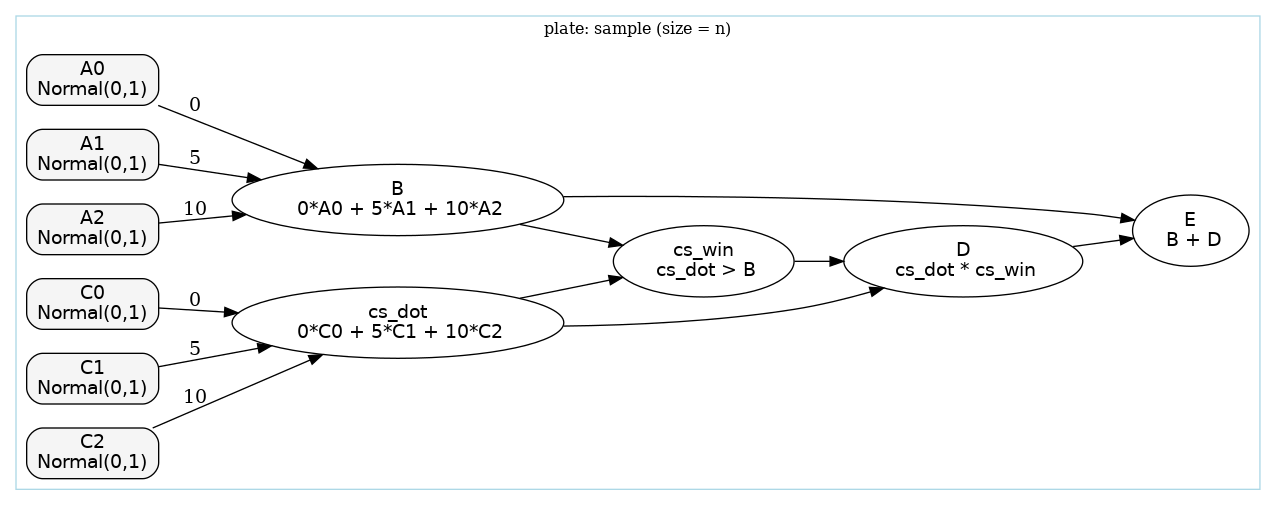
\includegraphics[width= 11cm]{figures/synthetic_causal_model.png}
\caption{Synthetic model involving overdetermination and undercutting used in the evaluation loop.}
\label{fig:synthetic_model}
\end{figure}


\begin{figure}
    \centering
    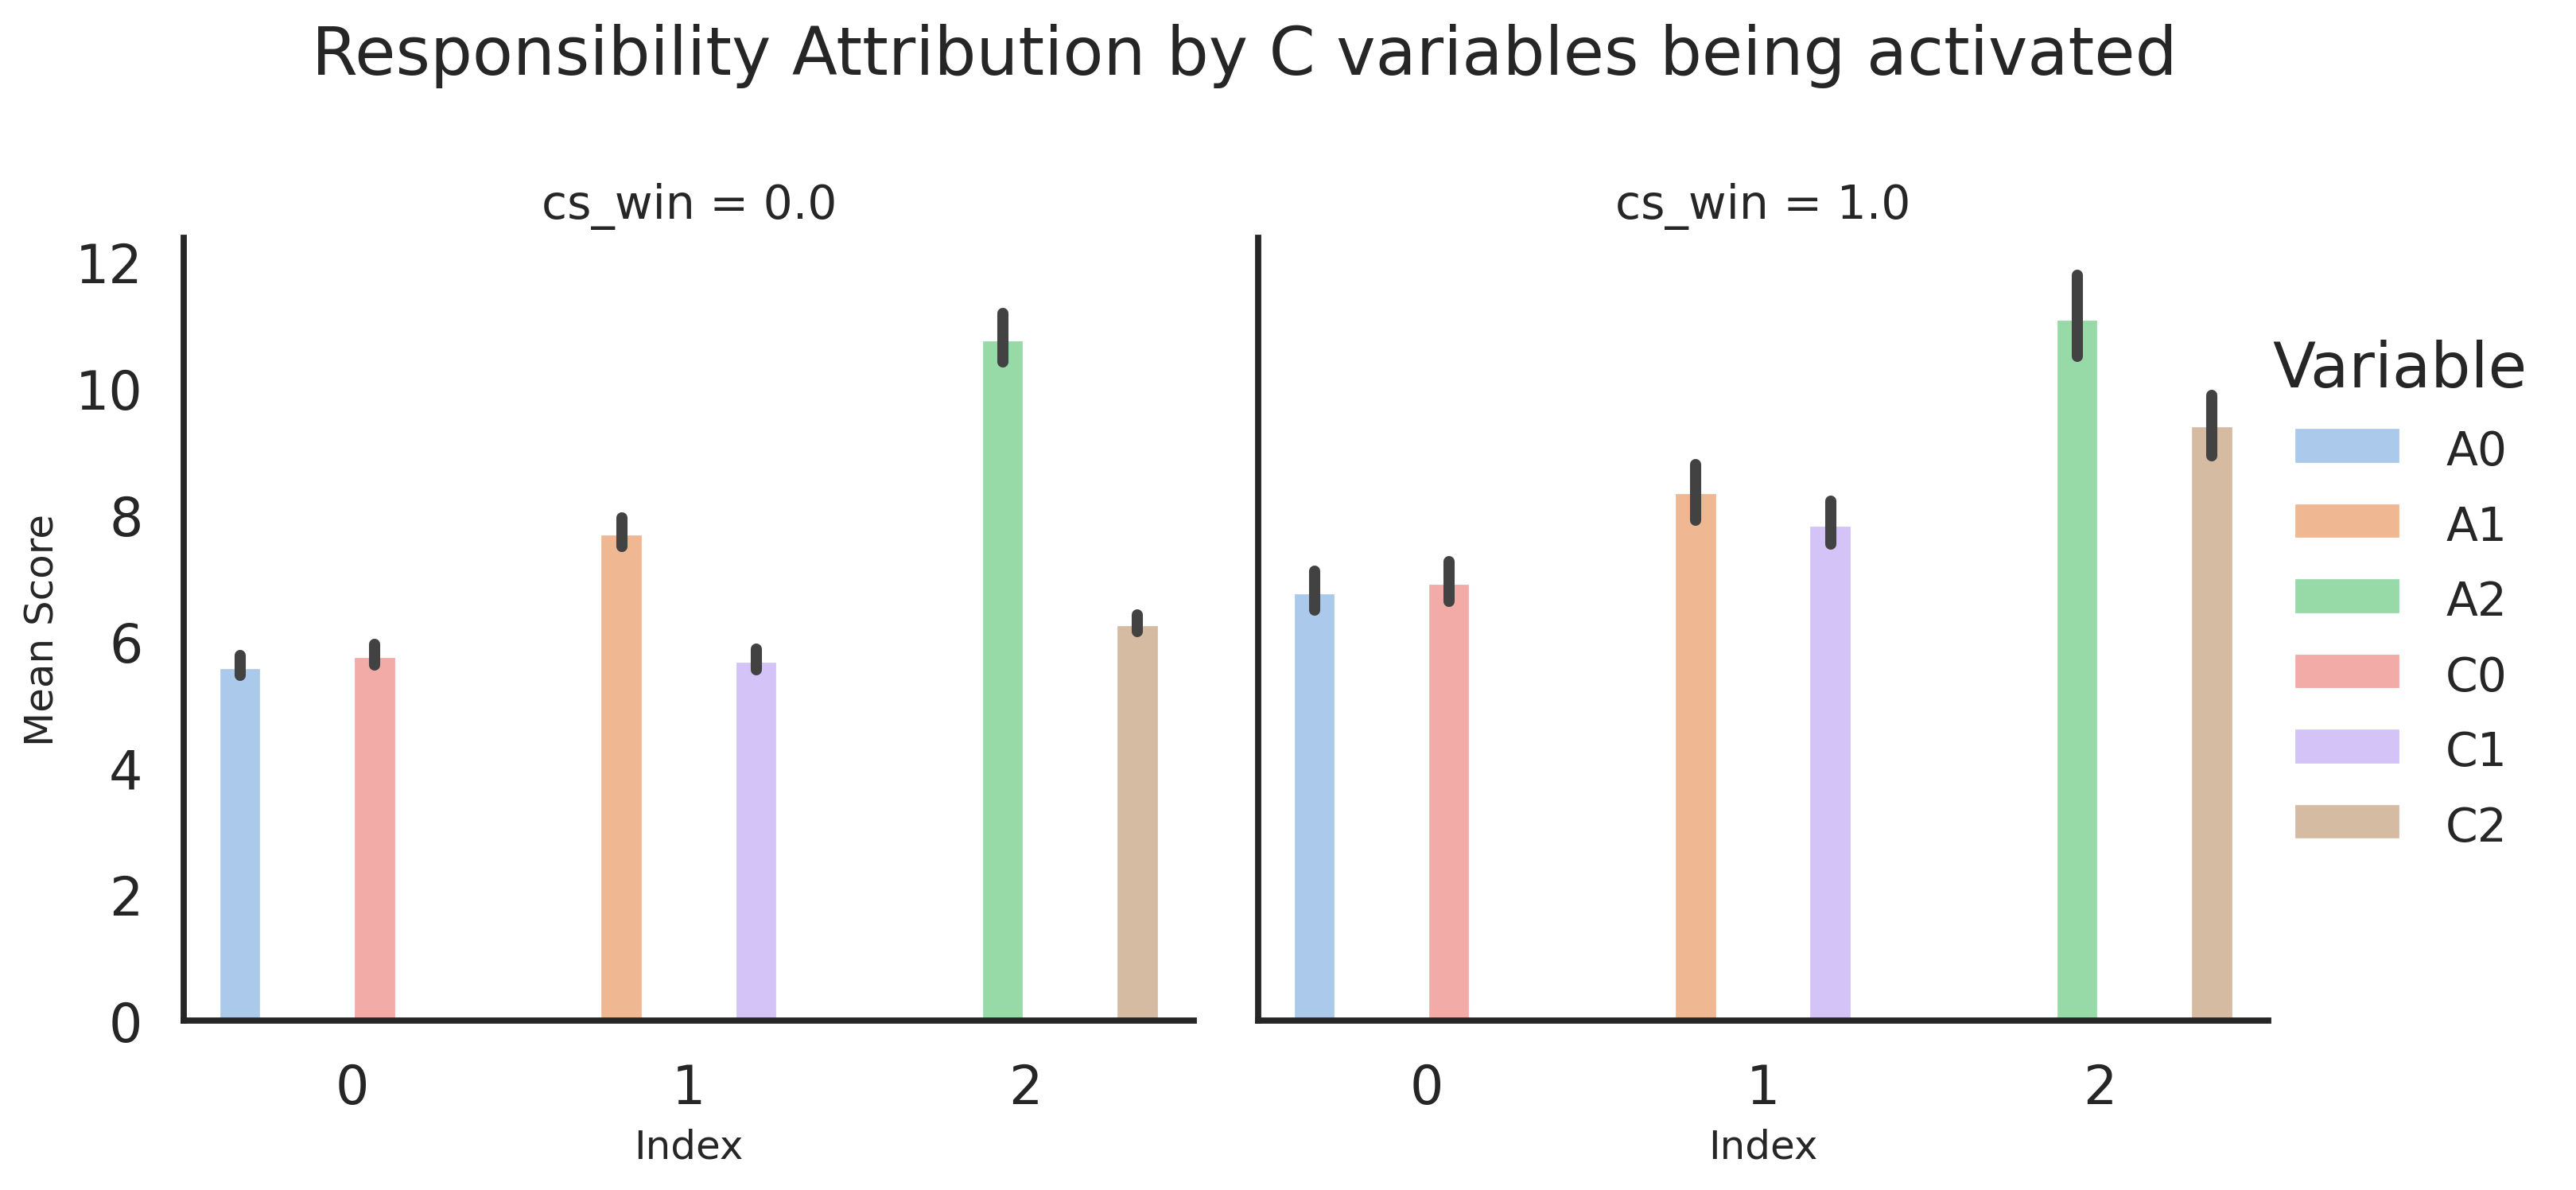
\includegraphics[width=0.9\linewidth]{figures/synthetic_causal_model_responsibility_attribution.png}
    \caption{Mean attribution scores to all upstream features in the synthetic model, 500 individual explanations, all based on a single search sample of size 5000. When `cs\_win=0', the $C$ variables are not activated, and so we expect total scores for all of them to be similar (red, violet, dark brown on the left-hand side). We still expect the scores for $A0$, $A1$, and $A2$ generally to increase independently of what happens with the $C$ variables, which we see on both sides (blue, light brown, and green on both sides). We also expect the scores for $C$ variables to increase if they are activated (red, violet, dark brown on the right-hand side). These expectations are satisfied.}
    \label{fig:synthetic_attribution}
\end{figure}


\begin{figure}
    \centering
    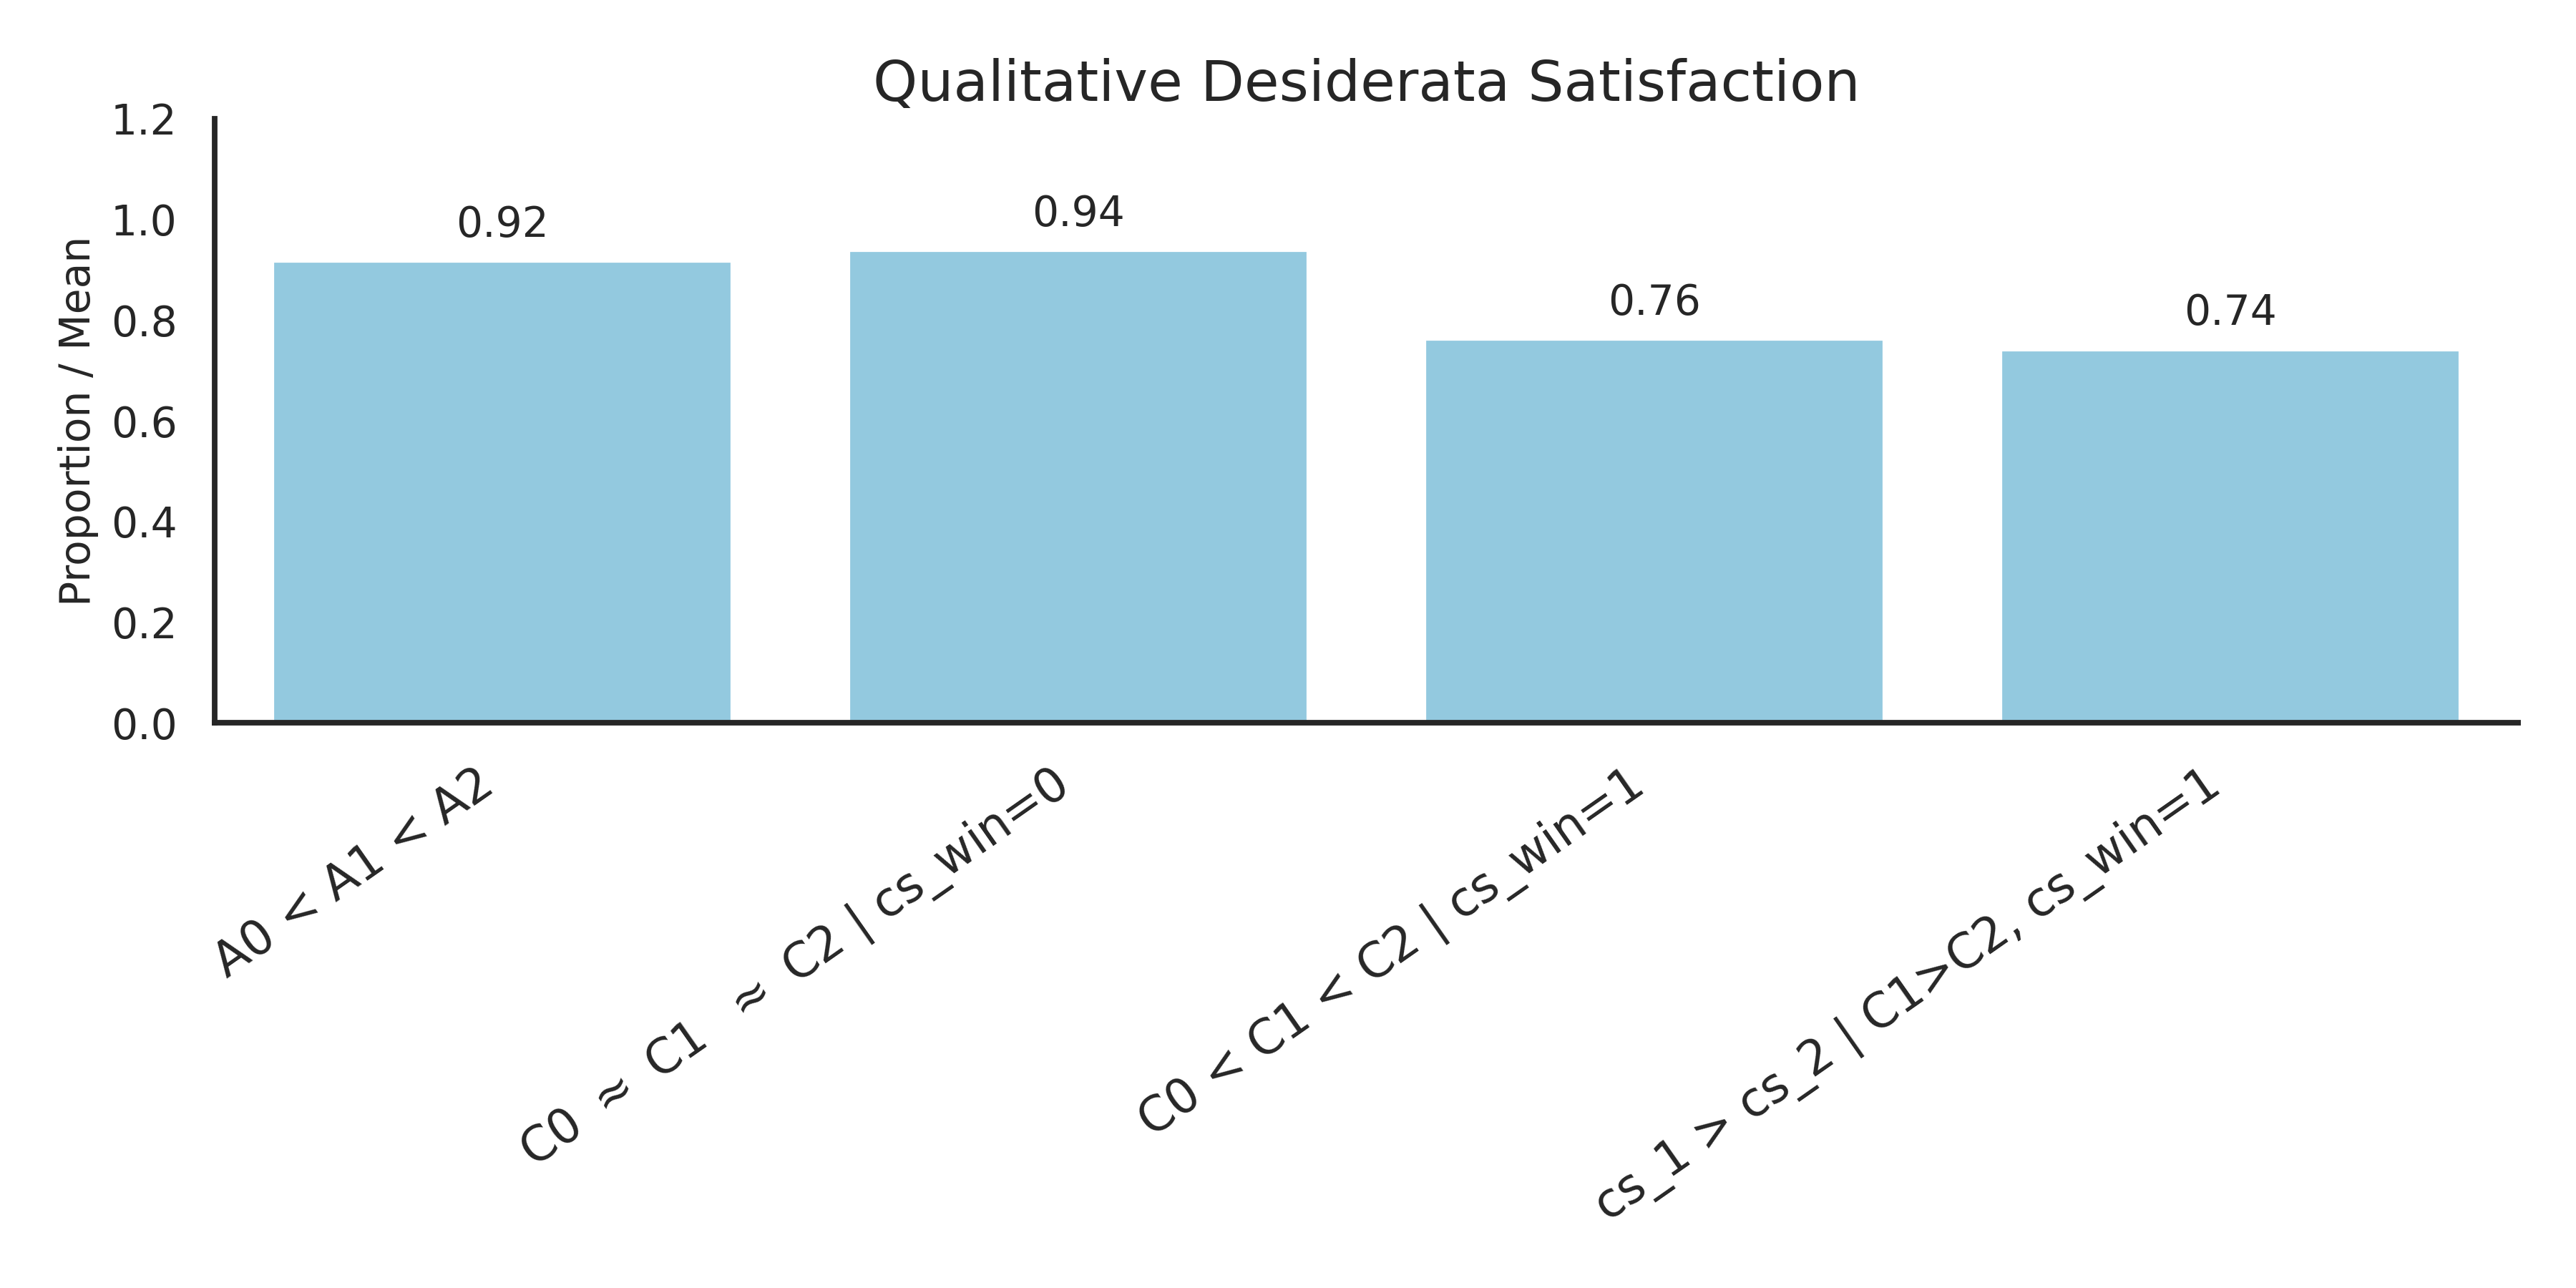
\includegraphics[width=0.9\linewidth]{figures/synthetic_causal_model_summary.png}
    \caption{Qualitative claims satisfaction frequency for causal attribution in the synthetic model, 500 local explanations all based on a single search sample of size 5000. Most of the time, the ordering of the scores for $A$ variables agrees with the ordering of the coefficients. Most of the time, close proximity of scores for inactive $C$ variables is quite high; most often, the ordering for active $C$ variables agrees with the ordering of the coefficients. We do not, however, want an explanation to track coefficients only, which, for instance, is illustrated by the last statement: if scores are reversed, this is mostly due to the disparate direction of the difference between the variable values.}
    \label{fig:synthetic_summary}
\end{figure}
